\documentclass{beamer}


\usepackage{beamerthemesplit}
\usepackage{latexsym,amssymb}
\usepackage[croatian]{babel}
\usepackage[]{algorithm2e}
\usepackage{graphicx}
\usepackage{hyperref}
\usepackage{color}
\usepackage{multirow}

%\setbeamercovered{transparent}
\setbeamertemplate{blocks}[rounded][shadow=true]

\usetheme{CambridgeUS}
%\usetheme{Boadilla}
\usecolortheme{beaver} %za crvenu nijansu te teme

\newcommand{\ncm}{\newcommand}
\ncm{\lb}{\label} \ncm{\puta}{\cdot } \ncm{\R}{\mathbb R}
\ncm{\Z}{\mathbb Z} \ncm{\N}{\mathbb N} \ncm{\C}{\mathbb C}
\ncm{\Q}{\mathbb Q} \ncm{\T}{\mathbb T} \ncm{\ch }{\' c} \ncm{\bl
}{$\blacktriangleright \:$} \ncm{\follows }{$\Rightarrow $}
\ncm{\ra}{\rightarrow} \ncm{\e }{{\rm e}}



\hyphenation{auto-mor-phism }


\newenvironment{jbam}{\begin{eqnarray*}}{\end{eqnarray*}}
\newenvironment{jbams}{\begin{eqnarray}}{\end{eqnarray}}


\def\rmdj {d\llap{\raise 1.22ex\hbox
  {\vrule height 0.09ex width 0.315em}\kern 0.04em}}
\def\sldj {d\llap{\raise 1.22ex\hbox
  {\vrule height 0.09ex width 0.265em}}\rlap{\raise 1.22ex\hbox
  {\vrule height 0.09ex width 0.05em}}}
\def\itdj {d\llap{\raise 1.22ex\hbox
  {\vrule height 0.09ex width 0.2em}}\rlap{\raise 1.22ex\hbox
  {\vrule height 0.09ex width 0.06em}}}
\def\bfdj {d\llap{\raise 1.16ex\hbox
  {\vrule height 0.126ex width 0.308em}\kern 0.04em}}
\def\ttdj {\rlap{\kern 0.17em\raise 1.1ex\hbox
  {\vrule height 0.09ex width 0.295em}}d}
\def\scdj {\rlap{\kern 0.04em\raise 0.57ex\hbox
  {\vrule height 0.09ex width 0.20em}}d}
\def\sfdj {d\llap{\raise 1.22ex\hbox
  {\vrule height 0.10ex width 0.3em}\kern 0.02em}}

\def\dj{\ifcase\fam \rmdj \or \or \or
  \or \itdj \or \sldj \or \bfdj \or \ttdj \or \sfdj \or \scdj \else \rmdj \fi}

\def\rmDj {\rlap{\kern 0.05em\raise 0.76ex\hbox
  {\vrule height 0.10ex width 0.28em}}D}
\def\slDj {\rlap{\kern 0.1em\raise 0.76ex\hbox
  {\vrule height 0.1ex width 0.28em}}D}
\def\itDj {\rlap{\kern 0.145em\raise 0.76ex\hbox
  {\vrule height 0.1ex width 0.274em}}D}
\def\bfDj {\rlap{\kern 0.044em\raise 0.72ex\hbox
  {\vrule height 0.126ex width 0.287em}}D}
\def\ttDj {\rlap{\kern 0.02em\raise 0.67ex\hbox
  {\vrule height 0.105ex width 0.20em}}D}
\def\scDj {\rlap{\kern 0.08em\raise 0.73ex\hbox
  {\vrule height 0.12ex width 0.24em}}D}
\def\sfDj {\rlap{\kern 0.02em\raise 0.727ex\hbox
  {\vrule height 0.126ex width 0.26em}}D}

\def\Dj{\ifcase\fam \rmDj \or \or \or
  \or \itDj \or \slDj \or \bfDj \or \ttDj \or \sfDj \or \scDj \else \rmDj \fi}



\title[Usporedba algoritama]{Usporedba algoritama baziranih na roju pri tra\v zenju globalnih ekstrema}
\author{Marko Stojanovi\' c,\\ Vanja Vukovi\' c}



\begin{document}

\frame{\titlepage}
\frame{\tableofcontents}

\section{Osnovni pojmovi i problematika}
\frame{
  \frametitle{Problem globalnog optimuma za nelinarne probleme}
  Dvije osnovne vrste problema:
  \begin{itemize}
   \item tra\v zenje optimuma na segmentu domene (npr. Schafferova F6 funkcija na $[-100,100]^2$)
   \item tra\v zenje optimuma funkcija ograni\v cenih sa nekim jednakostima i/ili nejednakostima na cijeloj domeni (npr. G funkcije).
  \end{itemize}
}

\frame {
  \frametitle{Meta-heuristike}
\begin{itemize}
  \item Meta-heuristike su strategije koje efikasno pretra\v zuju prostor rje\v senja te pronalaze ona rje\v senja koja su blizu optimalnih.
  \item Postoje dvije glavne glavne podjele metaheuristika:
  \begin{itemize}
   \item strategija pretra\v zivanja
    \begin{itemize}
    \item bazirane na lokalnom pretra\v zivanju
    \item bazirane na komponentama koje {\em u\v ce}
    \end{itemize}
    \item dimenzija
    \begin{itemize}
     \item jedno rje\v senje
     \item skup mogu\' cih rje\v senja.
    \end{itemize}
  \end{itemize}
\end{itemize}
}

\frame{
  \frametitle{Populacijski algoritmi}
  \begin{itemize}
   \item Velika klasa algoritama:
   \begin{itemize}
    \item evolucijski algoritmi, genetski algoritmi, PSO, $\dots$
   \end{itemize}
   \item Algoritmi bazirani na rojevima (eng. swarm intelligence) su podklasa populacijskih algoritama koji se oslanjaju na kolektivno pona\v sanje decentraliziranih i samostalnih \v cestica ili jedinki u roju.
   \item Primjer takvih algoritama su: PSO, mravlji algoritam i p\v celinji algoritam.
  \end{itemize}
}


\section{U znanstvenoj i stru\v cnoj literaturi}
\frame{
  \frametitle{U znanstvenoj i stru\v cnoj literaturi}
  \begin{block}{}
    \begin{thebibliography}{1}
    \bibitem{ZC} {\sc W. Zhu, J. Curry}, {\em Parallel Ant Colony for Nonlinear Function Optimization with Graphics Hardware Acceleration}, Proceedings of the 2009 IEEE International Conference on Systems, Man, and Cybernetics (2009) 1803--1808
    \end{thebibliography}
  \end{block}
  \begin{itemize}
    \item Mravlji algoritam
    \item Ackley, Griewank, Penalty1, Penalty2, Quadratic, Rosenbrock, Rastrigin, Schwefel 1.2, Schwefel 2.22, Schwefel 2.21, Sphere, Step
  \end{itemize}
}

\frame{
  \frametitle{U znanstvenoj i stru\v cnoj literaturi}
  \begin{block}{}
    \begin{thebibliography}{1}
    \bibitem{B} {\sc B. Alatas}, {\em Chaotic bee colony algorithms for global numerical optimization}, Expert Systems with Applications 37 (2010) 5682--5687
    \end{thebibliography}
  \end{block}
  \begin{itemize}
    \item P\v celinji algoritam
    \item Griewank, Rosenbrock, Rastrigin
  \end{itemize}
}

\frame{
  \frametitle{U znanstvenoj i stru\v cnoj literaturi}
  \begin{block}{}
    \begin{thebibliography}{1}
    \bibitem{AM} {\sc F. Aghazadeh, M. R. Meybodi}, {\em Learning Bees Algorithm For optimization}, International Conference on Information and Intelligent Computing IPCSIT vol.18 (2011) 115--122
    \end{thebibliography}
  \end{block}
  \begin{itemize}
    \item P\v celinji algoritam
    \item De Jong\footnote{Postoji 5 De Jong funkcija: Sphere, Rosenbrock (Rosenbrock's vally), Step, Quadratic i Shekel's Foxholes} 1 i 2, Rastrigin, Ackley
  \end{itemize}
}

\frame{
  \frametitle{U znanstvenoj i stru\v cnoj literaturi}
  \begin{block}{}
    \begin{thebibliography}{1}
    \bibitem{ME} {\sc K. M. Malan, A. P. Engelbrecht}, {\em Characterising the searchability of continuous optimisation problems for PSO}, accepted for publication, Swarm Intelligence, SpringerLink vol.8 (2014)
    \end{thebibliography}
  \end{block}
  \begin{itemize}
    \item PSO
    \item Ackley, Griewank, Quadric, Rana, Rastrigin, Rosenbrock, Salomon, Spherical, Schwefel 2.26, Step
  \end{itemize}
}


\frame{
  \frametitle{U znanstvenoj i stru\v cnoj literaturi}
  \begin{block}{}
    \begin{thebibliography}{1}
    \bibitem{RY} {\sc R. Rahmani, R. Yusof}, {\em A new simple, fast and efficient algorithm for global optimization over continuous search-space problems: Radial Movement Optimization}, Applied Mathematics and Computation 248 (2014) 287--300
    \end{thebibliography}
  \end{block}
  \begin{itemize}
    \item RMO -- vrsta PSO algoritma
    \item De Jong 1-5, Schaffer F6, Rastrigin, Griewank, Hyper-Ellipsoid, Ackley
  \end{itemize}
}


\section{O projektnom zadatku}
\frame{
  \frametitle{Projektni zadatak}
  \begin{itemize}
   \item Implementacija 3 algoritama iz klase algoritama baziranih na roju (ABC, PSO, OPSO) u programskom jeziku C.
   \item Izv\v savanje programskog koda na apache serveru.
   \item Korisni\v cko su\v celje izra\dj eno web tehnologijama.
   \item Putem korisni\v ckog su\v celja korisnik mo\v ze odre\dj ivati neke zajedni\v cke (broj iteracija, testna funkcija) i neke specifi\v cne parametere (koeficijenti koji se koriste u algoritmu).
   \item Grafi\v cki prikaz rezultata.
  \end{itemize}
}

\section{Algoritmi}
\frame{
  \frametitle{P\v celinji algoritam (ABC) - 1}
  \begin{itemize}
   \item Algoritam predstavlja roj p\v cela koje tra\v ze nektar u cvijetnom polju.
   \item Puno paramatera:
   \begin{itemize}
    \item izvi\dj a\v ci,
    \item radilice (dva parametra),
    \item 'elitni' izvi\dj a\v ci $\subset$ izvi\dj a\v ci (dva parametra),
    \item veli\v cina okoline za pretra\v zivanje,
    \item dubina istra\v zivanje dane okoline.
   \end{itemize}
   \item Ne konvergira.
  \end{itemize}
}

\frame{
  \frametitle{P\v celinji algoritam (ABC) - 2}
  \begin{itemize}
   \item Nasumi\v cno odaberemo mjesto na kojem \' ce izvi\dj a\v ci tra\v ziti.
   \item U $\epsilon$ okolinu najboljih $e$ izvi\dj a\v ca (eltni) saljemo po $ne$ radilica, a u kolinu sljede\' cih $m$ najbojih \v saljemo po $nm$ radilica ($\epsilon = (|b_d|+|b_g|)/n$).
   \item $k$ 'poditeracija' pretra\v zujemo tu okolinu (fiksirana vrijednost u testiranju $k=10$).
   \begin{itemize}
    \item Ako je prona\dj ena bolja vrijednost u $\epsilon$ okolini, suzi okolinu $\epsilon = \epsilon * 0.8$
   \end{itemize}

   \item Zapamti najbolju vrijednost i ponovi ciklus.
  \end{itemize}

}

\frame{
  \frametitle{Particle swarm optimisation - 1}
  \begin{itemize}
   \item Algoritam se bazira na kretanju jata riba (i ptica).
   \item 4 promjenjiva parametra:
   \begin{itemize}
    \item broj \v cestica u roju,
    \item inercija \v cestice ($\omega$), osobna komponenta \v cestice ($\rho_p$), socijalna komponeta \v cestice ($\rho_g$).
   \end{itemize}
    \item Algoritam konvergira.
  \end{itemize}
}

\frame{
  \frametitle{Particle swarm optimisation - 2}
  \begin{itemize}
   \item[1.] Nasumi\v cno raspodijeli \v cestice po prostoru pretra\v zivanja i zadaj im brzinu
   \item[2.] Izra\v cunaj novu poziciju: $x_i+v_i \longmapsto x_i$
   \item[3.] Izra\v cinaj novu brzinu: $v_i=\omega v_{i,d}+\rho_p(p_i-x_i)+\rho_g(g-x_i)$
   \item[4.] Ako nije zadovoljen uvijet vrati se na 2.
  \end{itemize}
}

\frame{
  \frametitle{Orbital particle swarm optimisation - 1}
  \begin{itemize}
   \item Algoritam se zasniva na klasi\v cnom PSO algoritmu uz lokalnu pretragu kao u ABC.
   \item Uz varijable iz PSO algoritma dodana je i varijabla $\epsilon$ koja odre\dj uje okolinu za lokalno pretra\v zivanje za najbolju \v cesticu
   \item Lokalno pretra\v zivanje se vr\v si po orbitama dane \v cestice fiksiranjem jedne dimenzije i iteracijom po dimenzijama (za to\v cku u dimenziji 30 dobijemo 30 novih to\v caka)
  \end{itemize}
}

\frame{
  \frametitle{Orbital particle swarm optimisation - 2}
  \begin{itemize}
   \item[1.] Nasumi\v cno raspodijeli \v cestice po prostoru pretra\v zivanja i zadaj im brzinu
   \item[2.] Izra\v cunaj novu poziciju: $x_i+v_i \longmapsto x_i$
   \item[3.*] Za najbolju \v cesticu izvr\v si pretragu po orbitama
   \item[4.] Izra\v cinaj novu brzinu: $v_i=\omega v_{i,d}+\rho_p(p_i-x_i)+\rho_g(g-x_i)$
   \item[5.] Ako nije zadovoljen uvijet vrati se na 2.
  \end{itemize}
}

\section{Testiranje i primjeri testnih funkcija}
\frame{
  \frametitle{Uvjeti testiranja}
  \begin{itemize}
   \item 4 jezgreni 64-bitni Intel procesor
   \item 8Gb RAM
   \item Linux operacijski sustav (2.6 kernel)
   \item Programski jezik C (kod prilagoden za 64-bitni sustav)
   \item Mersenne Twister generator pseudo-slu\v cajnih brojeva (procesorsko vrijeme se koristi kao 'sjeme' za genereiranje)
   \item Apache2 server
   \item web tehnologije: Php i JavaScript
  \end{itemize}
}

\frame{
 \frametitle{Parametri pri testiranju }
 \begin{itemize}
  \item Broj \v cestica $n$=50, 100, 150, 200 za svaki algoritam
  \item ABC: $m=\lfloor\frac{n}{2}\rfloor, e=\lfloor\frac{m}{2}\rfloor, ne=10, nm=5, \epsilon$ varijabilni
  \item PSO: $\omega=0.9, \rho_p=1, \rho_g=0.9$
  \item OPSO: $\omega=0.9, \rho_p=1, \rho_g=0.9 \epsilon=1$
  
 \end{itemize}
}

\frame{
  \frametitle{Primjeri testnih funkcija - Sfera (De Jong 1)}
  $$f(x)=\sum_{i=1}^{3}x_i^2, x\in \mathbb{R}^3, x_i \in [-5.12,5.12]$$
   \begin{center}
      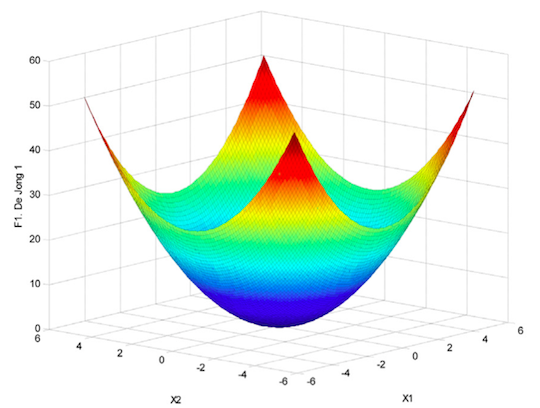
\includegraphics[scale=0.4]{imagestex/funkcija1.png}\\
   \end{center}
}

\frame{
  \frametitle{Primjeri testnih funkcija - Step (De Jong 3)}
  $$f(x)=\sum_{i=1}^{5}\lfloor x_i\rfloor, x\in \mathbb{R}^5, x_i \in [-5.12,5.12]$$
  \begin{center}
    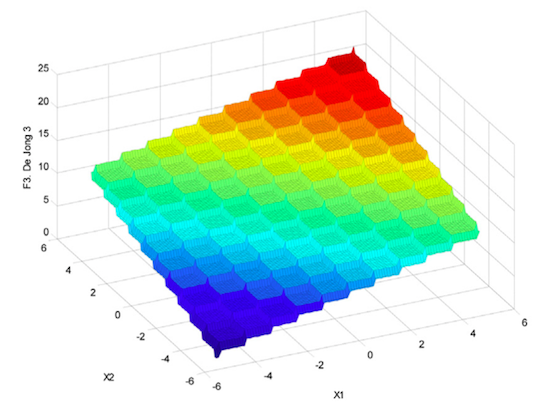
\includegraphics[scale=0.4]{imagestex/funkcija3.png}\\
  \end{center}
}

\frame{
  \frametitle{Primjeri testnih funkcija - Schaffer F6}
$$f(x)=0.5+\frac{sin^2(\sqrt{x_1^2 + x_2^2})-0.5}{[1+0.001 \cdot (x_1^2 + x_2^2)]^2}, x\in \mathbb{R}^2, (x_i)\in [-100,100]$$
  \begin{center}
    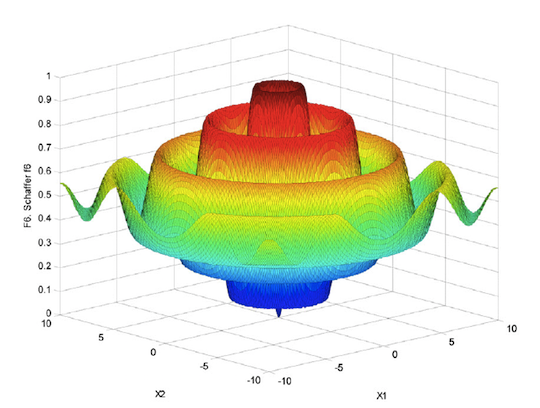
\includegraphics[scale=0.4]{imagestex/funkcija6.png}\\
   \end{center}
}

\frame{
  \frametitle{Primjeri testnih funkcija - Ackley}
 $$f(x) = -20\cdot exp\bigg(-0.2 \sqrt{\frac{1}{30} \sum_{i=1}^{30} x_i^2}\bigg) - exp\bigg(\frac{1}{30} \sum_{i=1}^{30} cos(2\pi x_i)\bigg) + 20 + e$$
 $$x\in \mathbb{R}^{30}, x_i\in [-30, 30]$$
  \begin{center}
    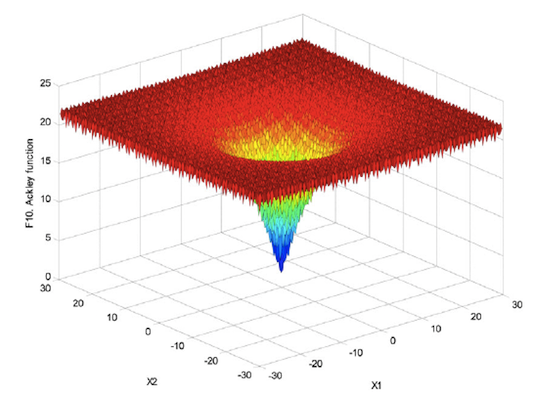
\includegraphics[scale=0.3]{imagestex/funkcija10.png}\\
  \end{center}
  }

\section{Rezultati testiranja}
%\frame{
%  \frametitle{Tabli\v cni prikaz broja iteracija - 1}
%  \begin{tabular}{c|c|c|c|c|c}
%        & De Jong 1 & De Jong 2 & De Jong 3 & De Jong 4 & De Jong 5\\ \hline
%   ABC  &  &   &   &   &   \\ \hline
%   PSO  &  &   &   &   &   \\ \hline
%   OPSO &  &   &   &   &   
%  \end{tabular}
%}

%\frame{
%  \frametitle{Tabli\v cni prikaz broja iteracija - 2}
%  \begin{tabular}{c|c|c|c|c|c}
%        & Schaffer F6 & Rastrigin & Griewank & Hyper-Ellipsoid & Ackley\\ \hline
%   ABC  &   &   &   &   &   \\ \hline
%   PSO  &   &   &   &   &   \\ \hline
%   OPSO &   &   &   &   &   
%  \end{tabular}
%}

\frame{
  \frametitle{Tabli\v cni prikaz broja iteracija - izbor}
  \begin{center}
  \begin{tabular}{c|c|c|c|c}
        & Sfera & Step & Schaffer F6 &  Ackley\\ \hline
   \multirow{4}{*}{ABC} & 38.03 & 475.53 & \color{green}{2} & N/A\\  
   	& 224.60 & 355.93 & \color{green}{1.93} & N/A\\
   	& 447.23 & 273.33 & \color{green}{2.70} & N/A\\
   	& 630 & 323.20 & \color{green}{2.57} & N/A\\ \hline
   \multirow{4}{*}{PSO} & 50.73 & 350.33 & 234.30 & 10 000 \\ 
    & 51.67 & 15.80 & 130.03 & 10 000 \\
    & 52 & 16.63 & 135.07 & 10 000 \\
    & 53.5 & 14.10 & 118.30 & 10 000 \\\hline
  \multirow{4}{*}{OPSO} & \color{green}{28.63} & \color{green}{6.27} & 76.83 & 8678.27\\
    & \color{green}{25.73} & \color{green}{4.83} & 51.97 & 4378.37\\
    & \color{green}{23.67} & \color{green}{4.87} & 36.13 & 2714.97\\
    & \color{green}{25.73} & \color{green}{4.87} & 38.4 & 1393.00 \\
  \end{tabular}
  \end{center}
}

\frame{
  \frametitle{Grafi\v cki prikaz prikaz - 1}
  \begin{center}
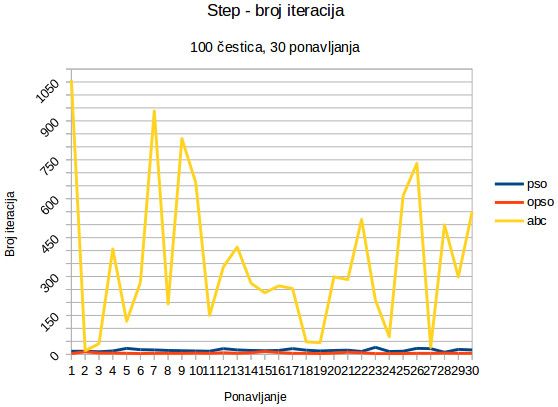
\includegraphics[scale=0.5]{imagestex/stepbriter.jpg}\\
\end{center}
  
}

\frame{
  \frametitle{Grafi\v cki prikaz prikaz - 2}
  \begin{center}
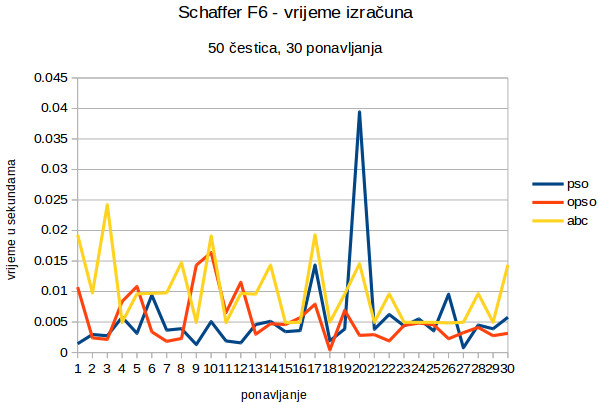
\includegraphics[scale=0.5]{imagestex/f6vrijeme.jpg}\\
\end{center}
  
}



\section{Grafi\v cko su\v celje}
\frame{
  \frametitle{Tehnologije}
  \begin{itemize}
   \item Php i Javascript skriptni jezici
   \item Php funkcija \emph{exec()} za poziv programa sa danim parametrima
   \item JavaScript funkcije za iscrtavanje grafova dobivenih rezultata
   \item Dva glavna dijela:
   \begin{itemize}
    \item odabir funkcije i varijabli
    \item grafički prikaz rezultata
   \end{itemize}

  \end{itemize}
}

\frame{
  \frametitle{Upotreba}
  \begin{itemize}
   \item Korisnik unese parametre u za to predvi\dj en prostor, uzimaju\' ci u obzir granice koje program prihva\' ca
   \item Klikom na gumb \emph{Po\v salji} poziva se \emph{exec()} koja se nalazi u drugom php modulu
   \item Korisnik \v ceka da se zavr\v se izra\v cuni nakon \v cega se fokusira dio stranice sa grafovima koji prikazuju dobivene rezultate
  \end{itemize}
}

\section{Literatura}
\frame{
  \frametitle{Literatira}
  \begin{thebibliography}{100}
    \bibitem{RY} {\sc R. Rahmani, R. Yusof}, {\em A new simple, fast and efficient algorithm for global optimization over continuous search-space problems: Radial Movement Optimization}, Applied Mathematics and Computation 248 (2014) 287--300
    \bibitem{AM} {\sc F. Aghazadeh, M. R. Meybodi}, {\em Learning Bees Algorithm For optimization}, International Conference on Information and Intelligent Computing IPCSIT vol.18 (2011) 115--122
    \bibitem{knj1} {\sc S. Luke}, {\em Essentials of Metaheuristics}, Lulu, second edition, \url{http://cs.gmu.edu/~sean/book/metaheuristics/}
     \bibitem{knj2} {\sc Z. Michalewicz, D. B. Fogel},{\em How to Solve It: Modern Heuristics}, Springer-Verlag Berlin Heidelberg (2000) 
  
    \bibitem{wiki}{\url{en.wikipedia.org/wiki/Particle_swarm_optimization}}, listopad 2014.
  \end{thebibliography}
}

\frame{
%  \frametitle{Literatira}
  \begin{thebibliography}{100}
    \bibitem{ZC} {\sc W. Zhu, J. Curry}, {\em Parallel Ant Colony for Nonlinear Function Optimization with Graphics Hardware Acceleration}, Proceedings of the 2009 IEEE International Conference on Systems, Man, and Cybernetics (2009) 1803--1808
\bibitem{B} {\sc B. Alatas}, {\em Chaotic bee colony algorithms for global numerical optimization}, Expert Systems with Applications 37 (2010) 5682--5687
\bibitem{AM} {\sc F. Aghazadeh, M. R. Meybodi}, {\em Learning Bees Algorithm For optimization}, International Conference on Information and Intelligent Computing IPCSIT vol.18 (2011) 115--122
\bibitem{ME} {\sc K. M. Malan, A. P. Engelbrecht}, {\em Characterising the searchability of continuous optimisation problems for PSO}, accepted for publication, Swarm Intelligence, SpringerLink vol.8 (2014)
  \end{thebibliography}
}



\end{document}
